\documentclass{article}%\documentclass[a4paper,10pt]{scrartcl}

%\usepackage[active,pdftex,tightpage]{preview}
\usepackage{tikz}

%\PreviewEnvironment{tikzpicture}

\usetikzlibrary{calc}

\begin{document}
%\maketitle

\section{lição 1}

Atividade 1 - página xx

\pagestyle{empty}
 \begin{tikzpicture}[scale=1.4]
  \draw (0,0) rectangle (1,6);
  \draw (1,0) rectangle (2,6);
  \draw (2,0) rectangle (3,6);
  \draw (3,0) rectangle (4,6);
  \draw (5,0) rectangle (9,3);
  \draw (5,0) rectangle (9,6);
  \draw (5,0) -- (9,3);
  \draw (5,3) -- (9,6);
\end{tikzpicture}
\vspace{0.5cm}

\begin{tikzpicture}[scale=1.4]
  \draw (0,0) rectangle (4,1.5);
  \draw (0,1.5) rectangle (4,3);
  \draw(0,3) rectangle (4,4.5);
  \draw(0,4.5) rectangle (4,6);
  \draw(5,0) rectangle (9,3);
  \draw(5,0) rectangle (9,6);
  \draw(7,0) -- (7,6);  
\end{tikzpicture}

\clearpage
 \begin{tikzpicture}[scale=1.4]
  \draw (10,0) rectangle (14,3);
  \draw (10,3) rectangle (14,6);
  \draw(12,0) -- (12,3);
  \draw(10,4.5) -- (14,4.5);
  \draw(15,0) rectangle (19,3);
  \draw(15,3) rectangle (19,6);
  \draw(15,1.5) -- (19,1.5);
  \draw(15,3) -- (19,6);
\end{tikzpicture}
\vspace{0.5cm}

\begin{tikzpicture}[scale=1.4]
  \draw (10,0) rectangle (14,3);
  \draw (10,3) rectangle (14,6);
  \draw (12,0) -- (12,3);
  \draw (10,3) -- (14,6);
  \draw (15,0) rectangle (19,3);
  \draw (15,3) rectangle (19,6);
  \draw (15,0) -- (19,3);
  \draw (19,3) -- (15,6);
\end{tikzpicture}



Atividade 9 (ativ meioemeio)


%retângulos

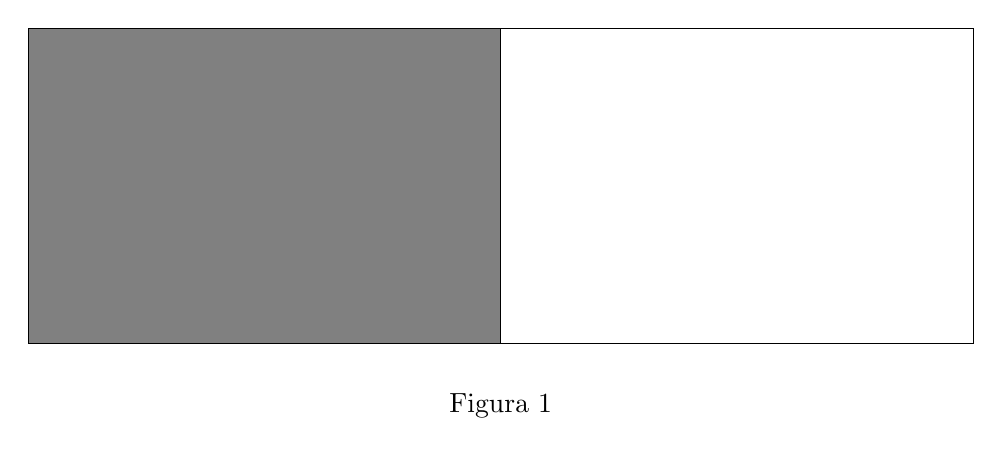
\begin{tikzpicture}[scale=2]
 \draw[fill=gray] (0,0) rectangle (3,2);
 \draw (3,0) rectangle (6,2) (3,-0.4) node{Figura 1};
\end{tikzpicture}

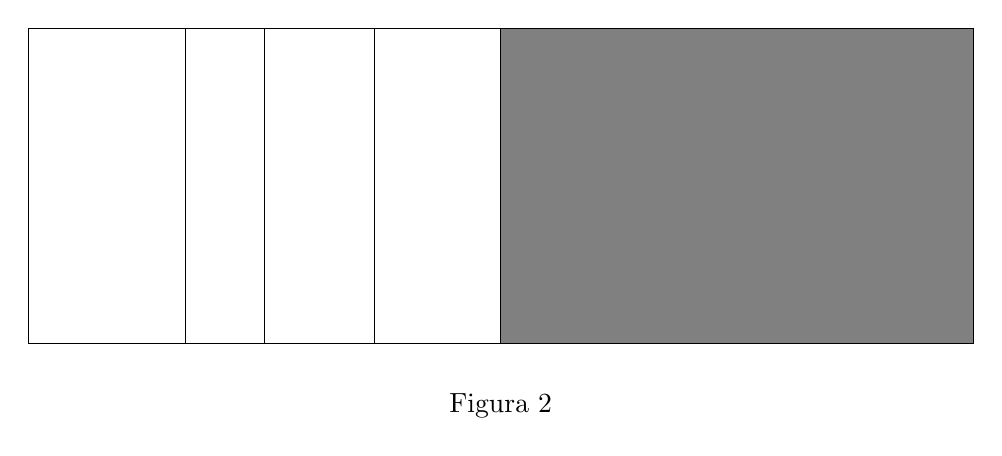
\begin{tikzpicture}[scale=2]
 \draw (0,0) rectangle (3,2);
 \draw (1,0) -- (1,2);
 \draw (1.5,0) -- (1.5,2);
 \draw (2.2,0) -- (2.2,2);
 \draw[fill=gray] (3,0) rectangle (6,2) (3,-0.4) node{Figura 2};
\end{tikzpicture}

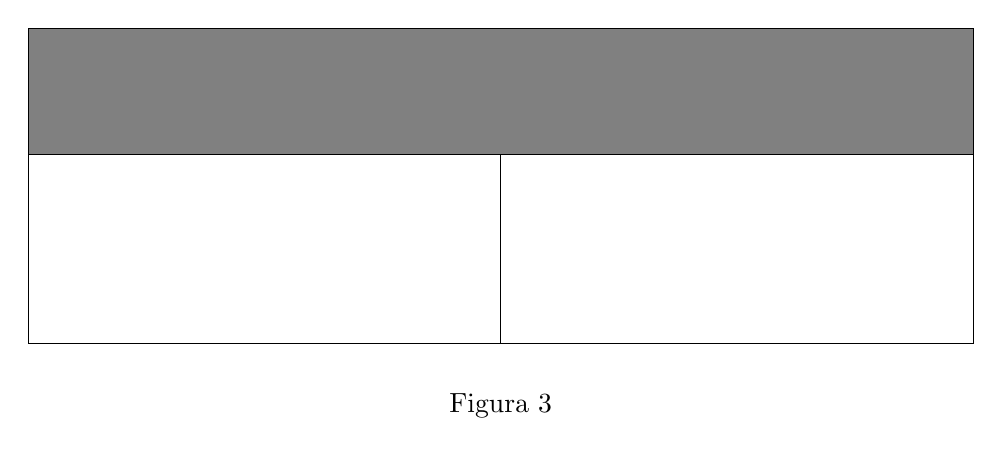
\begin{tikzpicture}[scale=2]
 \draw (0,0) rectangle (3,2);
 \draw (3,0) rectangle (6,2) (3,-0.4) node{Figura 3};
 \draw[fill=gray] (0,2) rectangle (6,1.2);
 \end{tikzpicture}

 % círculos

 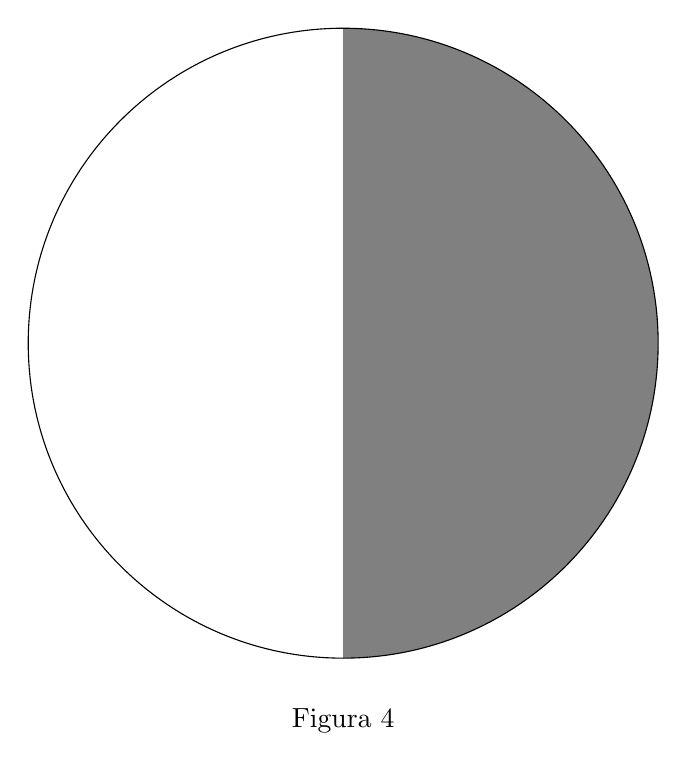
\begin{tikzpicture}[scale=2]
 \draw[fill=gray] (0,-2) arc (-90:90: 2);
 \draw (0,2) arc (90:270:2) (0,-2.4) node{Figura 4};
\end{tikzpicture}

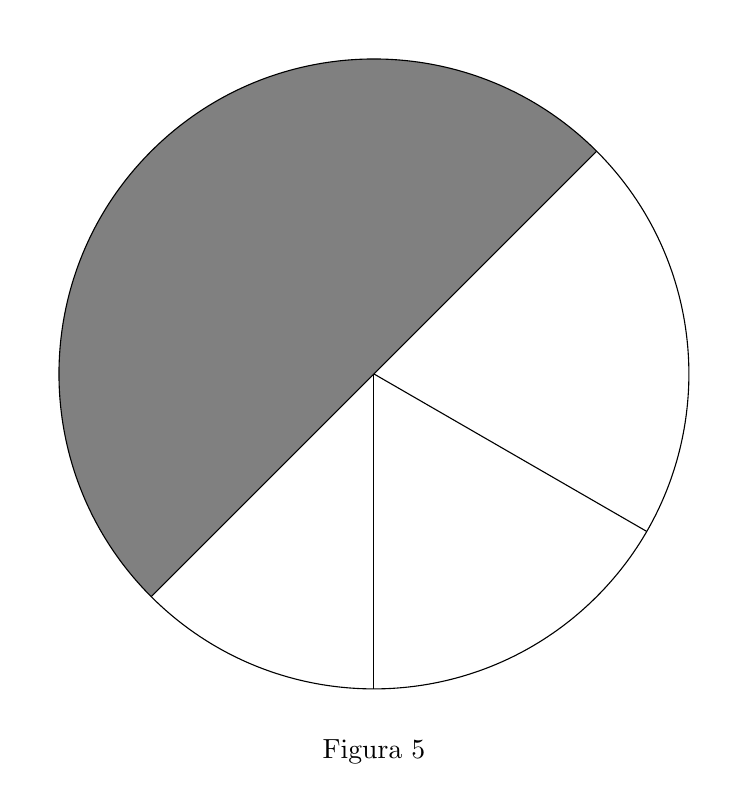
\begin{tikzpicture}[scale=2]
 \draw[fill=gray] (45:2) arc (45:225:2);
 \draw (225:2) arc (225:405:2) (0,-2.4) node{Figura 5};
 \draw (0,0) -- (0,-2);
 \draw (0,0) -- (-30:2);
 \draw (225:2) -- (45:2);
 \end{tikzpicture}

 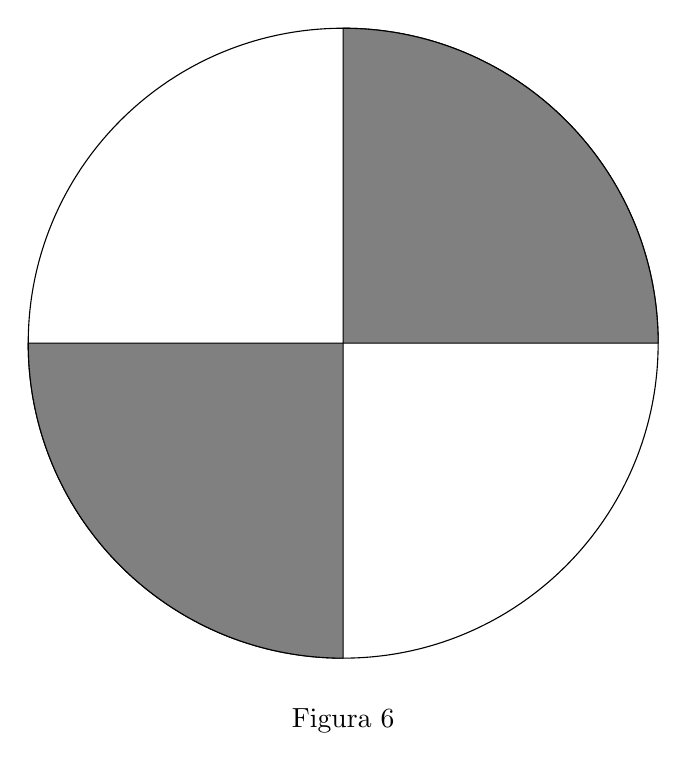
\begin{tikzpicture}[scale=2]
 \draw (0,0) circle (2);
 \draw[fill=gray] (0,0) -- (2,0) arc (0:90:2) -- cycle; 
 \draw[fill=gray] (0,0) -- (-2,0) arc (180:270: 2) -- cycle;
 \node at (0,-2.4) {Figura 6};
\end{tikzpicture} 

% hexágonos

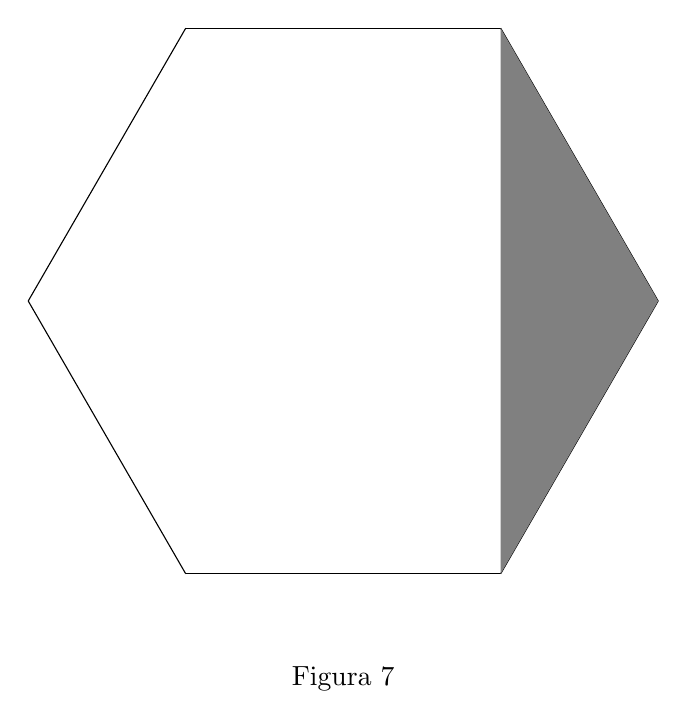
\begin{tikzpicture}[scale=2]
 \foreach \x in {0,60,...,300}{
 \draw (\x:2) -- (\x +60: 2);}
 \fill[gray] (2,0) -- (60:2) -- (300:2);
 \node at (0,-2.4) {Figura 7};
\end{tikzpicture}

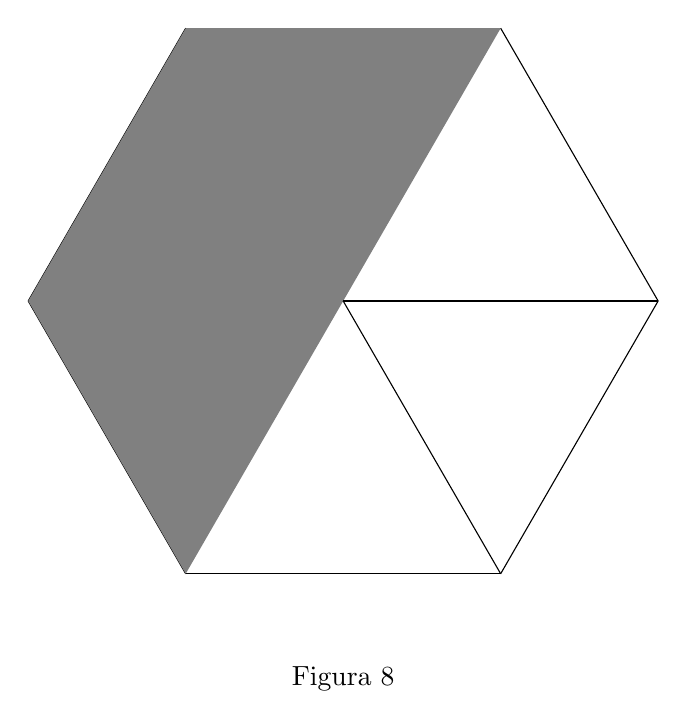
\begin{tikzpicture}[scale=2]
 \foreach \x in {0,60,...,300}{
 \draw (\x:2) -- (\x +60: 2);}
 \fill[gray] (60:2) -- (120:2) -- (180:2) -- (240:2) --cycle;
 \draw (0,0) -- (2,0);
 \draw (0,0) -- (300:2) (0,-2.4) node{Figura 8};
\end{tikzpicture}

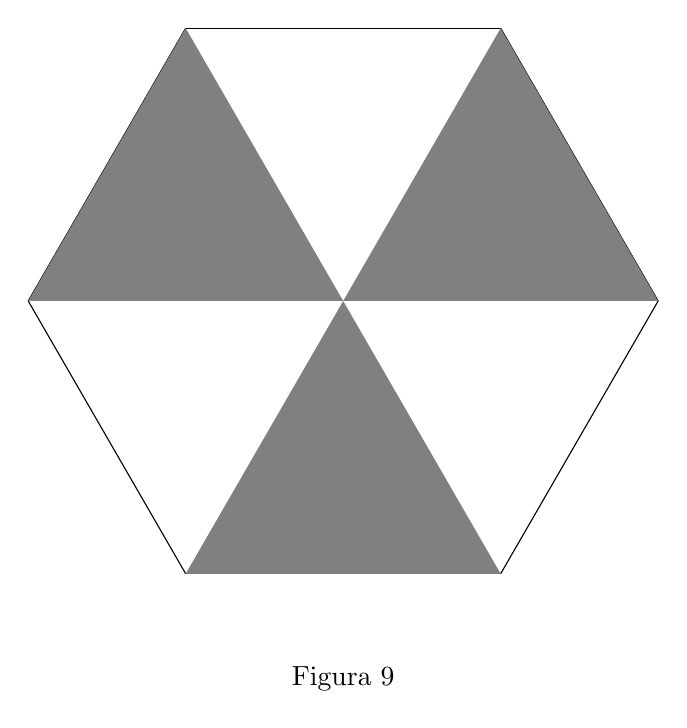
\begin{tikzpicture}[scale=2]
 \foreach \x in {0,60,...,300}{
 \draw (\x:2) -- (\x +60: 2);}
 \fill[gray] (0:2) -- (60:2) -- (0:0) --cycle;
 \fill[gray] (120:2) -- (180:2) -- (0:0) --cycle;
 \fill[gray] (240:2) -- (300:2) -- (0:0) --cycle;
 \node at (0,-2.4) {Figura 9};
\end{tikzpicture}

%círculo

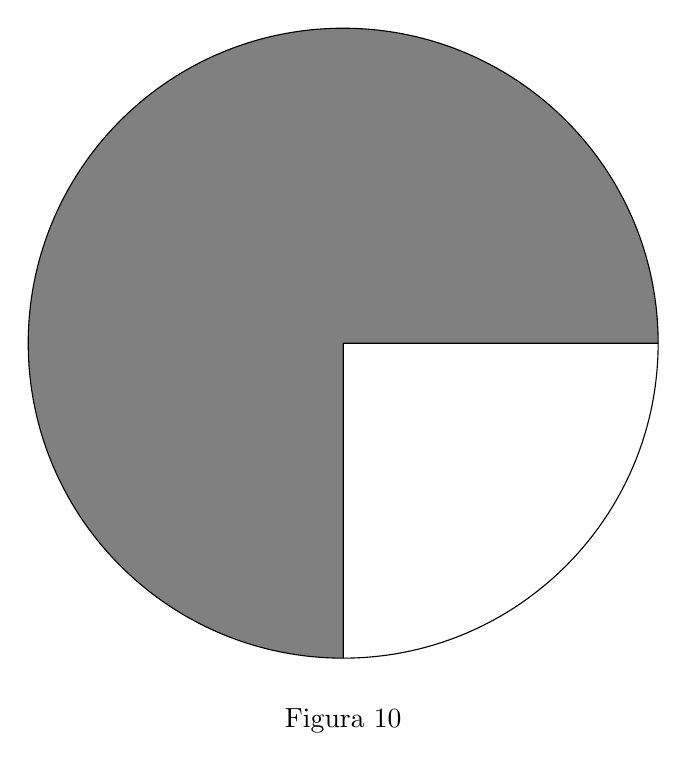
\begin{tikzpicture}[scale=2]
 \draw[fill=gray] (0:2) arc (0:270:2) -- (0,0) -- cycle;
 \draw (270:2) arc (270:360:2);
 \draw (0,0) -- (0,-2);
 \draw (0,0) -- (2,0)  (0,-2.4) node{Figura 10};
 \end{tikzpicture}

%hexágonos

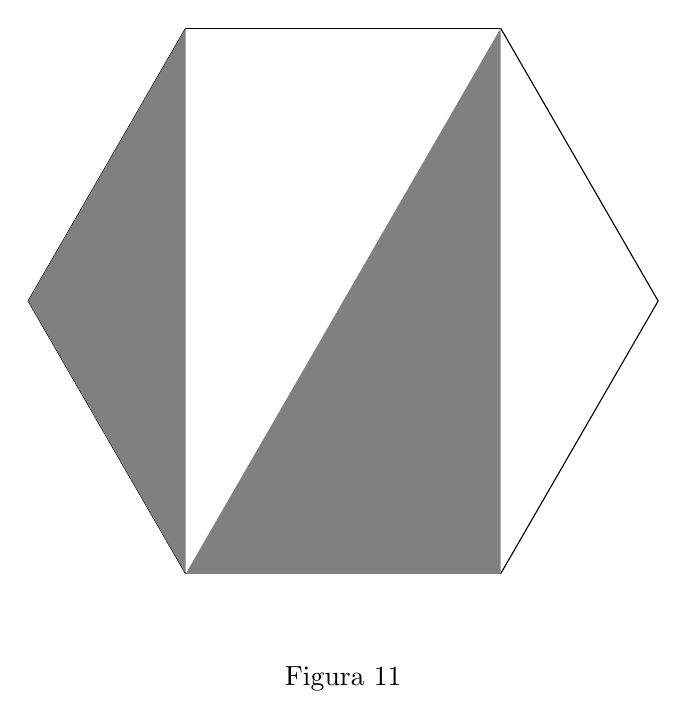
\begin{tikzpicture}[scale=2]
 \foreach \x in {0,60,...,300}{
 \draw (\x:2) -- (\x +60: 2);}
\fill[gray] (120:2) -- (180:2) -- (240:2) -- cycle;
\fill[gray] (240:2) -- (300:2) -- (60:2) -- cycle;
 \node at (0,-2.4) {Figura 11};
\end{tikzpicture}

%retângulo
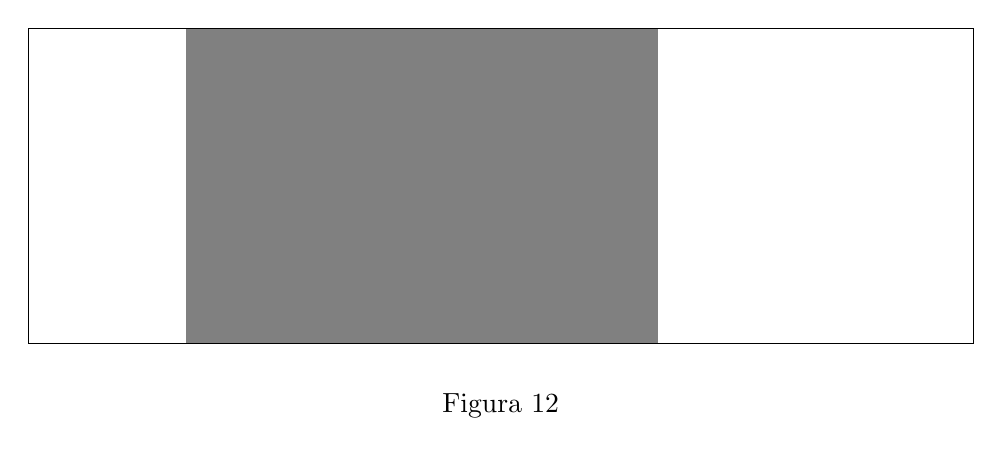
\begin{tikzpicture}[scale=2]
 \fill[gray] (1,0) rectangle (4,2);
 \draw (0,0) rectangle (6,2);
 \node at (3,-0.4) {Figura 12};
 \end{tikzpicture}

Atividade 11 ativ visual linguagem


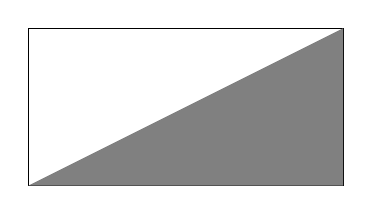
\begin{tikzpicture}
 \draw (0,0) rectangle (4,2);
 \fill[gray] (0,0) -- (4,2) -- (4,0) -- cycle;
\end{tikzpicture}

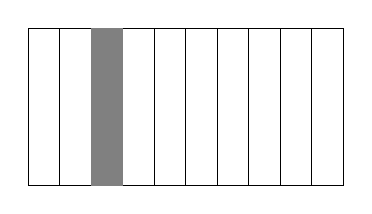
\begin{tikzpicture}
 \draw (0,0) rectangle (4,2);
 \foreach \n in {0.4,0.8,1.2,...,3.2,3.6}{
 \draw (\n,0) -- (\n,2);}
 \fill[gray] (0.8,0) -- (0.8,2) -- (1.2,2) -- (1.2,0) -- cycle;
\end{tikzpicture}


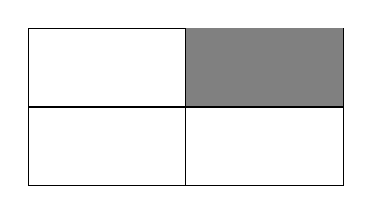
\begin{tikzpicture}
 \draw (0,0) rectangle (4,2);
 \fill[gray] (2,1) rectangle (4,2);
 \draw (0,1) -- (4,1);
 \draw (2,0) -- (2,2);
 \end{tikzpicture}

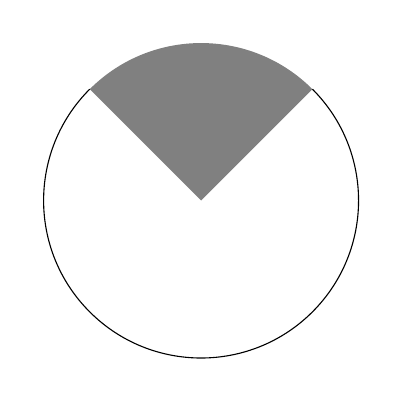
\begin{tikzpicture}
 \fill[gray] (45:2) arc (45:135:2) -- (0,0) -- cycle;
 \draw (135:2) arc (135:405:2);
\end{tikzpicture}
 

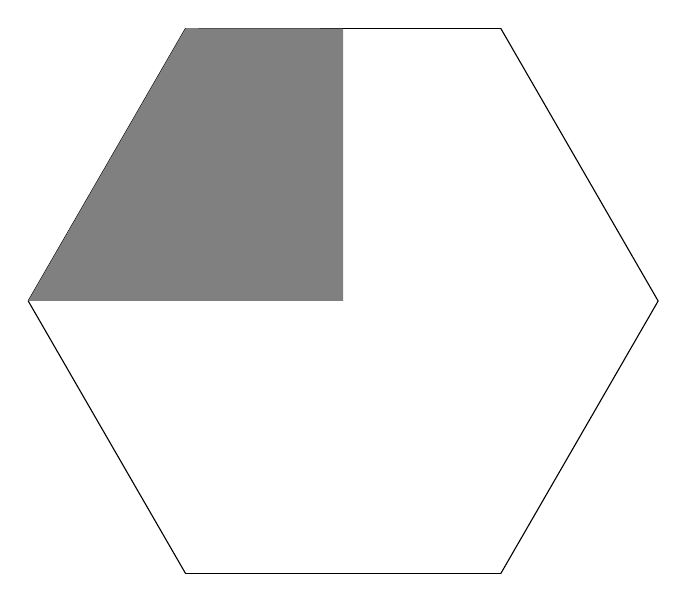
\begin{tikzpicture}[scale=2]
 \foreach \x in {0,60,...,300}{
 \draw (\x:2) -- (\x +60: 2);}
\fill[gray] (-2,0) -- (0,0) -- (0,1.73) -- (120:2) -- cycle;
\end{tikzpicture}

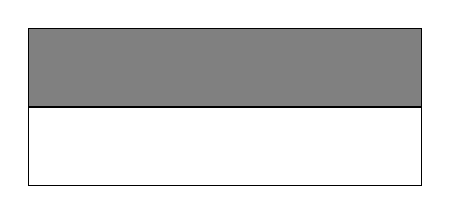
\begin{tikzpicture}
 \draw (0,0) rectangle (5,1);
 \draw[fill=gray] (0,1) rectangle (5,2);
\end{tikzpicture}


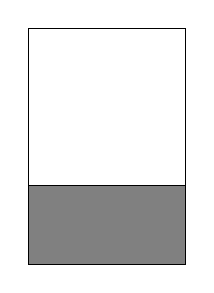
\begin{tikzpicture}
 \draw[fill=gray] (0,0) rectangle (2,1);
 \draw (0,1) rectangle (2,3);
\end{tikzpicture} 


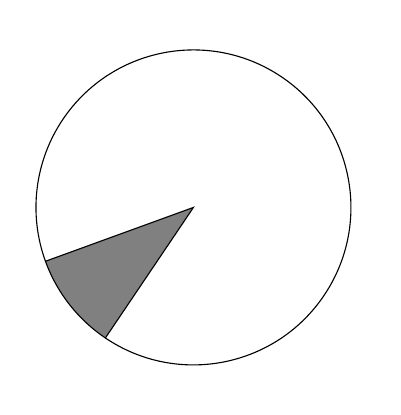
\begin{tikzpicture}
 \draw[fill=gray] (200:2) arc (200:236:2) -- (0,0) -- cycle;
 \draw (236:2) arc (236:560:2);
\end{tikzpicture} 

%i)
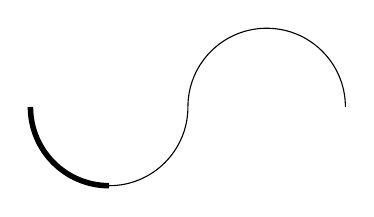
\begin{tikzpicture}
 \draw[line width=2pt] (-1,0) arc (180:270:1);
 \draw (0,-1) arc (270:360:1) -- (1,0) arc (180:0:1);
 \end{tikzpicture}

%j) paralelepípedo
\begin{tikzpicture}
    \pic [fill=gray] at (0,0) {annotated cuboid={width=5, height=10, depth=10}};
    \pic [fill=white] at (4.5,0) {annotated cuboid={width=45, height=10, depth=10}};
    \end{tikzpicture}


%l)
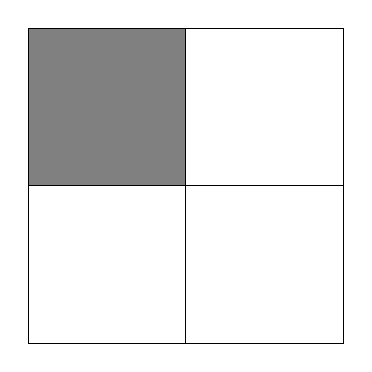
\begin{tikzpicture}
 \draw[fill=gray] (0,2) rectangle (2,4);
 \draw (0,0) rectangle (2,2);
 \draw (2,0) rectangle (4,2);
 \draw (2,2) rectangle (4,4);
 \end{tikzpicture} 

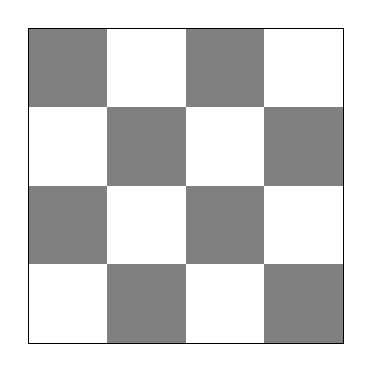
\begin{tikzpicture}
 \fill[gray] (1,0) rectangle (2,1);
 \fill[gray] (3,0) rectangle (4,1);
 \fill[gray] (0,1) rectangle (1,2);
 \fill[gray] (2,1) rectangle (3,2);
 \fill[gray] (1,2) rectangle (2,3);
 \fill[gray] (3,2) rectangle (4,3);
 \fill[gray] (0,3) rectangle (1,4);
 \fill[gray] (2,3) rectangle (3,4);
 \draw (0,0) rectangle (4,4);
\end{tikzpicture}

\section{licao 2}
\end{document}
